\section{(Linear) Auto-Encoders projecting to  In-Distribution subspace}

{\color{red}
Global upper bounds $\bar{\beta}$ obtained across the entire input space tend to be overly pessimistic on vanilla DNN, since they must accommodate all possible inputs, including inputs not In (training) Distribution (ID) \citet{OOD}. Such samples display large value for 
$x_C - x'_C + x'_D - x_D$, see Fig.~\ref{fig3} (left) for MNIST.
Considering the full input space on the original DNN will thus produce high global upper bounds $\bar{\beta}$, no matter the method employed. Restricting to ID inputs seems unpractical, as there is no established characterization of ID inputs. We propose an efficient alternative:
%To address this, we employ principal component analysis (PCA) \citet{Paco}, a technique from engineering science, to restrict the output (hence lowering the bounds) {\em without} restricting the input.
Extract the most important components of the ID dataset using an Auto-Encoder (AE), and project away the other components from an input before feeding it to the DNN. In practice, we train the AE on the ID dataset to obtain the ID latentspace.
We then define the AE-DNN architecture as first using the AE-coder to reduce to the latent space, then use the decoder to go back to the full space (called projected input), and finally calling the DNN on the projected input, see Fig \ref{fig:AE-DNN}. 
%Such architecture has been used previously, e.g. by \citet{MEnet}, but for a different purpose.

%AE-DNN will behave largely as the original DNN on ID inputs. However, 
%
Computing bounds $\bar{\beta}$ on non-linear AE-DNN is more costly than on original DNN, as additional integer vairables are required. From now on, we consider {Linear AE-DNN (LAE-DNN)}.

%We construct the {\em PCA-DNN} by prepending PCA-encoding and decoding to the original DNN, transforming an image into its {\em PCA-representation}, see Fig.~\ref{fig.MNIST}.
%This reduced feature space retains the most important features of the dataset. 
Call $dim$ the dimension of the full space, and $n$ the size of the latent space of the LAE trained on an ID dataset. LAE-Decoding is a linear function. By optimality, it can be assumed to be of rank $n$: it defines $n$ linearly independent vetors of dimension $1 \times dim$.
%This set of $n$ vectors can be completed with $dim-n$ vectors into a basis of the full space. 
An optimal choice of LAE-encode is the projection of input to these $n$ vectors. That is, calling LAE-decode and LAE-encode projects away features not on the ID latent-space.
Hence, on ID inputs, LAE-DNN will behave largely as the original DNN. However, global bounds on the LAE-DNNs will be smaller than on the original DNN, because of the projection to the ID latent space.
Indeed, largest $x_C - x'_C + x'_D - x_D$ found 
on LAE-DNN is 6 times smaller than on DNN, and corresponds to more ID images, see Fig.~\ref{fig3} (right).


\begin{proposition}
 For all DNN and all latent space dimension $n$, $\beta^\varepsilon_{C,D}(\text{LAE-DNN}) \leq \beta^{\varepsilon}_{C,D}(\text{DNN})$.
\end{proposition}

In practice, the upper bound computed are better (3-15x) for LAE-DNN than for DNN (Section \ref{sec:realtime}).

\begin{figure*}[t!]
	\centering
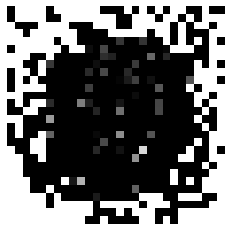
\includegraphics[scale=0.35]{image.png} 
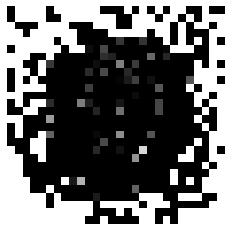
\includegraphics[scale=0.35]{perturb.png} \hspace{0.5cm}

\includegraphics[scale=0.3]{redimage.png}

\includegraphics[scale=0.3]{redperturb.png}
\caption{Left: pair (I,I') image and its perturbation (in a unique pixel at x=14, y=8 from top) maximizing $\underline{\beta}^{.5}_{6,8}=.518$ for DNN. Right: a pair (I,I') 
maximizing $\underline{\beta}^{.5}_{6,8}=.084$ for LAE-DNN.}
\label{fig3}
\end{figure*}	

\iffalse
\begin{figure*}[b!]
	\centering

\includegraphics[scale=0.35]{redimage.png} \hspace{1.5cm}

\includegraphics[scale=0.35]{redperturb.png}
\caption{An (ID) image for MNIST and its perturbation when using the PCA-representation, maximizing $\underline{\beta}^{.5}_{6,8} = .084$, as obtained by the{\em Diff} model.}
\vspace{-0.2cm}
\label{fig4}
\end{figure*}	
\fi



{\em Training:} LAE is trained on an ID dataset with several values of latent space $n$. We set the size $n$ by checking the accuracy of LAE-DNN, that is, the $\%$ of images where the predicted class matches the ground truth. We set $n$ as small as possible (for efficiency) while ensuring that the LAE-DNN accuracy loss is minimal ($ \leq 1 \%$) wrt the original DNN (20 for DNN=FC-MNIST). 
Such an $n$ exists as for $n=dim$ LAE-DNN=DNN.


Then, we compute bounds on LEA-DNN from the full input space, as described in the previous section. In exploitation, we call LEA-DNN on any given input, and use the global bound on LEA-DNN to 
do real-time robustnesss certification.
%The dataset input images are minimally changed by the PCA-encoding/decoding. 
%Although PCA-representations are full size (784 pixels for MNIST), they lie in a reduced space. 

\iffalse
\begin{figure*}[t!]
    \centering
    \vspace{-0.3cm}
    
\includegraphics[scale=0.75]{MNIST.pdf} 
    \caption{The pipeline training and exploiting the {\bf PCA-DNN} on MNIST dataset.}
    \label{fig.MNIST}
\end{figure*}	


we treat the pixels of the original image $I$ and the perturbed image $I'$ as variables, along with the reduced PCA dimensions ($20 \times 2$ from $I$ and $I'$). These are then fed to the first layer of the DNN (linear transformation). 
%Compared to computing bounds on the original DNN, we only add {\em linear} variables, as few as 2x the reduced PCA dimensions.
The associated constraints, which come from the PCA-encode/decode, are also linear. Next, we have the exact same MILP encoding (e.g., {\em Diff} encoding) for the DNN. Hence, the number of {\em binary} variables for PCA-DNN is the same as without PCA. Finally, the goal is to optimize, e.g., $\beta^\varepsilon_{6,8}$, the value of $y_6 - y_8 = x_6 - x'_6 + x'_8 - x_8$,  where $y_C$ is the {\em diff} variable of the output neuron for class $C \in \{6, 8\}$.

We report in Fig.~\ref{fig3} the image and perturbed image reaching the maximal lower bound $\underline{\beta}^{.5}_{6,8}=0.518$ 
obtained when using the original DNN (without PCA).
They are OOD inputs to the MNIST digit classification dataset.
%
In contrast, there are natural (ID) images and perturbed images 
reaching the maximal lower bound $\underline{\beta}^{.5}_{6,8}=0.084$ 
of the {\em  PCA-DNN} (Fig.~\ref{fig4}): among all the images producing a given worst-case PCA-representation, we can choose the PCA-representation itself, which is ID.
% This occurs because the output of the PCA-encoding/decoding (from reduced space) is its own image, and thus can be used as original input, producing the maximal $\underline{\beta}_{6,8}=.084$.
Note that the lower bound $\underline{\beta}$ is lower for the PCA-DNN, which is perfectly normal as we restrict the network's {\em output} to a reduced space close to the MNIST dataset. This will also be the case for the upper bound $\overline{\beta}$, which is very desirable as it improves robustness certification. 
%On the other hand, 

\fi



%
%It was also used to obtain the PCA encoding and decoding, transforming the images into a reduced basis. The number of PCA dimensions was chosen such that the exploitation accuracy remains constant. That is, encoding into a PCA basis and decoding it results in the same accuracy, as illustrated in ``Exploitation''. 
%
%Last, for the ``bound computation'', we determine an $L_1$-perturbation $\varepsilon$. The search space for bound computation is 20-dimensional. However, the bound itself is computed on the full space. This is possible since PCA is a \emph{linear operation} based on the eigenvectors of the covariance matrix and its transpose for the PCA decoding (inverse).


}